\thispagestyle{empty}
\begin{center}
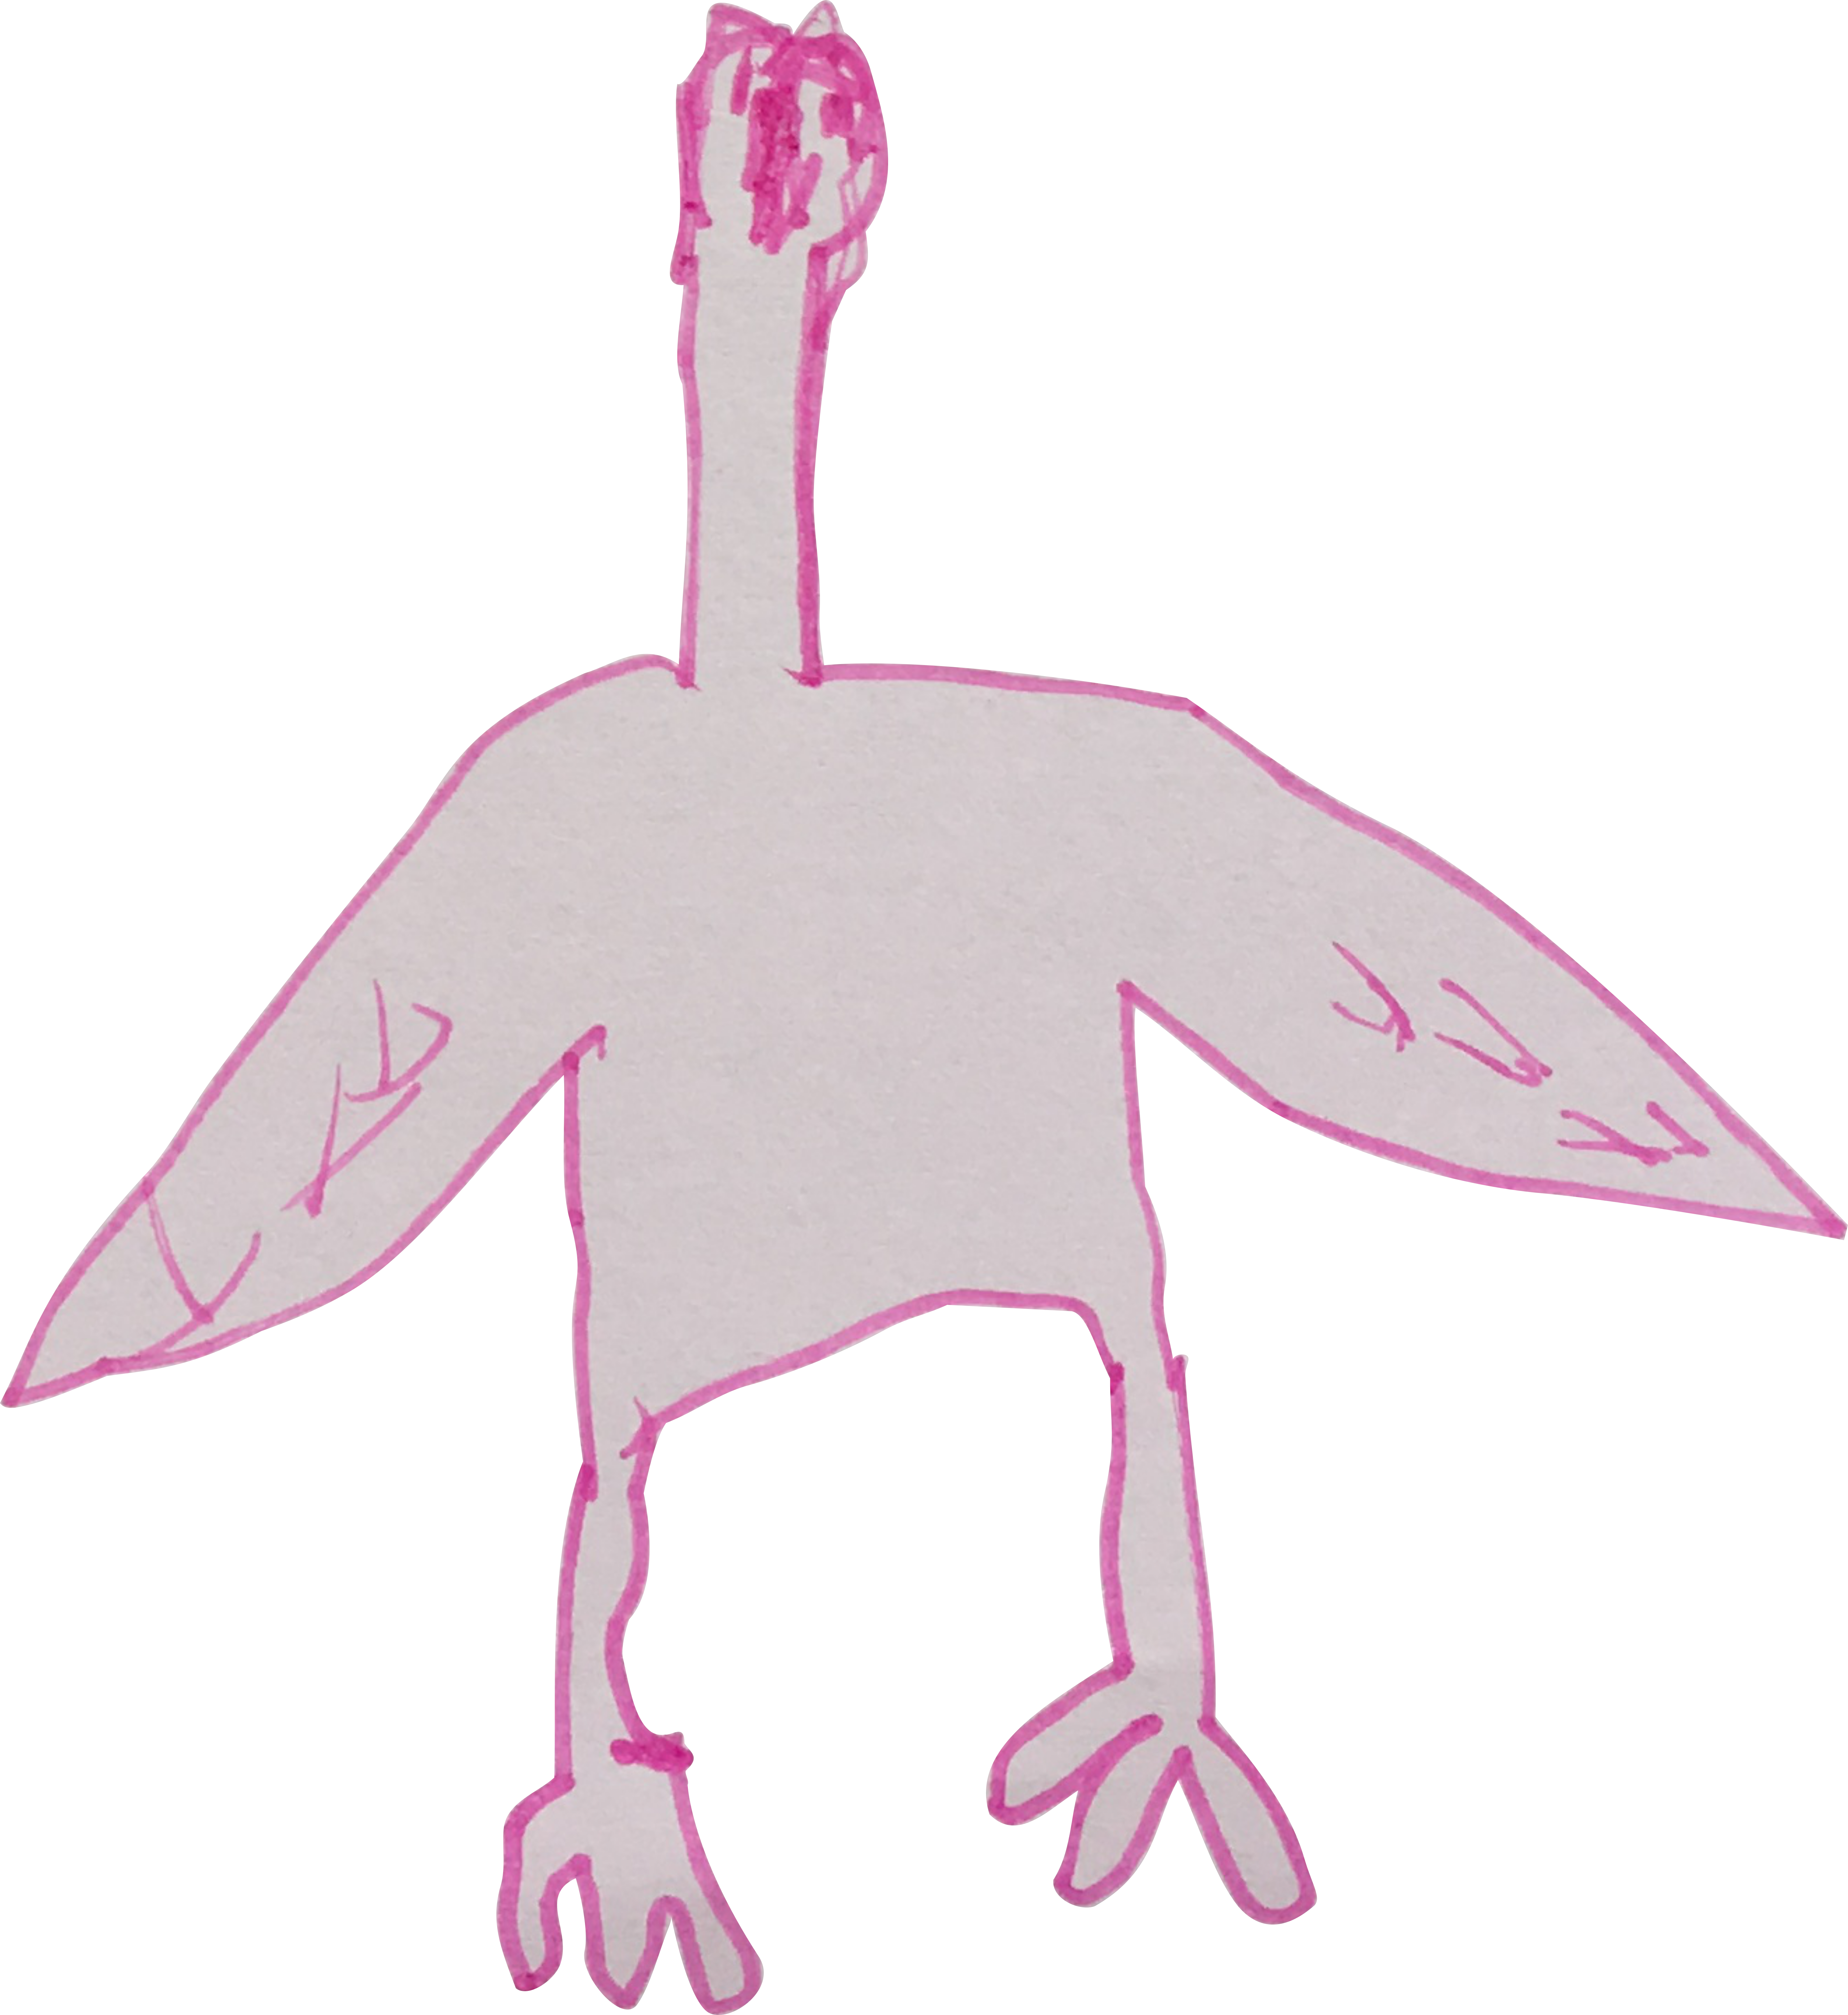
\includegraphics[height=.7\textheight]{./bilder/huhn2.png}
\end{center}
\vskip 2cm
{\Huge\color{farbe}\hfill{\tt{Hühner}}}
\addcontentsline{toc}{chapter}{Hühner}
\newpage
%%%%%%%%%%%%%%%%%%%%%%%%%%%%%%%%%%%%%%%%%%%%%%%%%%%%%%%%%%%%%%%%%%%%%%%%%%%%%%%
\lettrine[lines=2, lhang=.2, loversize=.25, lraise=0.05, findent=0.1em,
nindent=0em]{W}{}ie jeden Sonntagmorgen streiten sich der Hahn Jan und die
Henne Johanna. Die anderen Hühner ziehen sich in solchen Momenten in die
hinterste Ecke des Hühnerhofs zurück und warten bis am Mittag die Bäuerin die
Essenreste bringt, dann ist meisten wieder Ruhe. 

Die Henne Johanna und der Hahn Jahn sind legen sehr viel Wert darauf, gebildet
zu sein und zeigen das auch gerne. Sie können leidenschaftlich ihre Meinung
vertreten, die aber immer genau das Gegenteil der Meinung des anderen ist. 

\enquote{Wenn due so schlau bist wie Du meinst, mein lieber Jan, dann verrate
mir doch mal, was zuerst da war, eine Hehnne oder ein Ei!}

Die Hehnne Johanna weiss natürlich, dass es gar nicht so einfach ist, dieses
Rätsel zu lösen und lächelt spöttisch. Das sieht natürlich niemand, ein Lächeln
zu zeigen, fällt Hühnern im Allgemeinen ziemlich schwer.


\enquote{Ach was für eine uninteressante Frage!} Hahn Jan kratzt auf dem Boden
herum, ob nicht vielleicht doch mal wieder ein Regenwurm in der Nähe ist. 

\enquote{Zuerst meine liebe Johanna, war weder ein Ei, noch eine Henne, sondern natürlich ein Hahn.}

Da die Henne Johanna nicht sofort antwortet, meint Hahn Jan schon, diese Runde
gewonnen zu haben, plustert die Brust und setzt hinzu:


\enquote{Und glaube mir, das waren glückliche Zeiten!}

Natürlich hat die Antwort Henne Johanna etwas überrascht, aber das darf man in
so einer Diskussion keinesfalls zeigen. Das wäre ja noch schöner.

\enquote{Da lachen ja die Hühner!}

Und tatsächlich lacht sie schallend, dass die anderen Hühner vor Schreck ganz
still stehen und die Köpfe ducken.


\enquote{Hähne mein Lieber, sind bekanntermassen die überflüssigsten Wesen.
Ausser über den Hof zu stolzieren und morgens laut zu krähen, seid ihr zu
nichts zu gebrauchen. Ich habe von Hühnerhöfen gehört, da lebt seit
Generationen kein Hahn mehr und es klappt dort trotzdem alles prima.}

Hahn Jan ist beleidigt und pickt sehr energisch auf dem Boden herum, obwohl
dort gar nichts ist. Vor sich hin schimpfend läuft er einmal dem Zaun entlang.


\enquote{Dann beantworte du mir doch mal eine Frage.}

Hahn Jan bringt die Flügel in eine Stellung, die eigentlich nur für
besonderen Gelegenheiten und grossen Feste reserviert ist.


\enquote{Wer war zuerst da, Hühner oder Bauern?}

Darüber hatte die Henne Johanna noch nie nachgedacht. Jetzt ist sie wirklich
still, weil ihr nichts einfällt. 

Die Glucke Gesine, die gerade mit ihren Kücken einen Spaziergang über den Hof
macht, hatte die letzte Frage gehört.

\enquote{Hat euch beiden Eure Mutter denn gar nichts beigebracht, oder habt ihr
schon wieder alles vergessen?}

Ohne eine Antwort der beiden Streithühner abzuwarten dreht sie sich zu ihren
Kücken um, ruft, dass der heutige Unterricht eben vorverlegt wird, denn hier
sei eine Bildungslücke, so gross wie der Apfelbaum. 

Die Kücken setzen sich, der Hahn Jan und die Henne Johanna setzen sich dazu und
die Glucke Gesine fängt an zu erklären:

\enquote{Alles, was geboren wird, braucht als erstes einmal Liebe. Ohne Liebe
lein Leben. So war es auch mit dem ersten und grössten Ei, unserer Erde.
Nachdem das Ei da war, schlüpften immer wieder neue Tiere aus ihm aus. Zuerst
die Hühner, dann die Gänse, dann die Spatzen und dann nach und nach alle
anderen Vögel.


Sie lebten glücklich und zufrieden nebeneinander, es war mehr als genug Futter
für alle da. Aber aus dem Ei schlüpften nach und nach immer mehr Tiere, auch
andere, die nicht fliegen konnten. Erst ein Vogel Strauss, dann Pinguine und
dann alle Arten von Fischen und Echsen und sonstigen Tieren. Aber das waren nur
die Tiere, die am Tag aus dem Ei kamen. Die, die nachts geboren werden, hatten
die anderen Tiere noch nicht bemerkt. 

Und mit diesen Tieren war das Glück auf Erden für immer vorbei. Schlangen
kamen, die die Eier aus den Nestern stahlen, Katzen, die die Kücken jagten. Und
in einer Nacht, so stürmisch das die Baumspitzen vom Wind bis auf den Boden
gedrückt wurden, wurde noch ein Brüderpaar geboren, so heimtückisch und
gefährlich wie noch keines vorher.

Es waren der Fuchs und der Marder. Sie kamen nachts, schlichen sich an und
frassen Hühner. Es war grausam. Sehr viele Hühner verloren ihr Leben.

Die Hühner hielten eine Versammlung ab. Von nah und fern kamen sie, um zu
beraten, was sie gegen diesen Feind unternehmen wollten. Viele tapfere
Ritterhühner und Ritterhähne waren schon in den Kampf gezogen, aber niemand war
zurückgekehrt.

Sie beschlossen Späher auszuschicken in die ganze Welt, jemanden zu suchen, der
ihnen gegen Fuchs und Marder helfen konnte. Die Bauern. Eine Henne, die
schlaueste von allen, wurde beauftragt, mit den Bauern zu verhandeln.

Sie ging zum Bauern und brachte ihm das wertvollste, dass sie besass. Ein Ei
aus ihrem Gelege. Die Bauern betrachteten das Ei von allen Seiten und zum
Schrecken der Henne zerschlugen sie es.

Ihr schien, als wären die Menschen die noch grösseren Barbaren als Fuchs und
Marder. Das innere des Eis landete auf einem heissen Stein, grad bei ihrem
Feuer. Die Bauern probierten und lachten und klopften sich gegenseitig auf die
Schultern.

Sie holten grosse Säcke aus den Scheunen und liefen los, die Hühner
einzufangen. Jedes einzelne Huhn wurde von Menschen gefangen. Aber welches
Wunder. Die Menschen frassen nur ganz wenige der Hühner. Den anderen bauten sie
einen Zaun, gross und stark genug, damit sie vor Fuchs und Marder geschützt
waren. 

Jeden Morgen brachten die Bauern frisches Futter, sogar im Winter. Aber der
Preis war hoch. Sie nahmen den Menschen von da an im Tausch für ihre Sicherheit
die Eier weg. Aber wir Hühner schafften es mit dem vielen Futter jeden Tag ein
Ei zu legen. Manche liessen die Bauern, damit neue Kücken ausgebrütet werden
konnten.

Und seitdem leben wir Hühner und die Bauern nebeneinander her und sorgen
füreinander. Die Eier gaben den Bauern Kraft und unsere Intelligenz. Sie fingen
an, grössere Häuser für uns zu bauen, wenn eine von uns krank wurde, kam ein
Bauer im weissen Kittel und half. 

Und eine Bäuerin, die ein besonders gutes Ei gegessen habe musste, hat sogar
die im winter beheizbare Wasserleitung direkt in den Hühnerstall erfunden. }




\enquote{}


\vfill
